
\section{Additional Experimental Results and Details}
\label{sec:appendix-experiments}

Here we provide additional details and results for the Transformer and MLP experiments discussed in Section~\ref{sec:experiments}.

\subsection{Transformer Experiments}
\label{sec:transformer-exp-details}

\paragraph{Parity task details} We follow the setting of \citet{shaw2024alta}. The train set consists of examples with lengths ranging from 1 to 20. The train set includes $100,000$ examples, with roughly an equal number of examples per number of ones. We evaluate out-of-distribution (OOD) accuracy on a test set with lengths ranging from 21 to 40. 

\paragraph{ALTA program for parity} The ALTA program for parity that we use for our manual initialization is based on the sequential algorithm with relative position representations presented in~\citet{shaw2024alta}. This algorithm computes parity by iterating through each position (one per layer), flipping a running parity
bit every time a one is encountered. We simply reverse the direction of iteration from left-to-right to right-to-left, to accommodate that our model's classification decision depends on the \texttt{SEP} token at the beginning of the input sequence (see below).

\paragraph{Architecture and ALTA weight conversion}
One implementation challenge is that our experiments require a trainable Transformer that is compatible with ALTA-compiled weights. The reference ALTA Transformer implementation in \texttt{numpy} is not trainable~\citep{shaw2024alta}. To accomplish this, we implement a trainable version in Jax~\citep{jax2018github}, following the same parameterization expected by the ALTA compiler. This parameterization uses relative position representations~\citep{shaw2018self} following the parameterization of T5~\citep{raffel2020exploring}, which uses a single scalar bias term for relative positions within some window. It also uses an alternative parameterization for the attention head output transformations, as proposed by~\citet{elhage2021mathematical}, to simplify compilation; however, this alternative attention output parameterization is shown to be equivalent to that of the original Transformer. We select the logits for the \texttt{SEP} token as the output of the model, as our experiments focus on classification tasks.

A more significant challenge is that ALTA-compiled weights are not designed to be used with layer normalization~\citep{ba2016layer}. As the sequential algorithm for parity requires at least as many layers as bits in the longest input sequence, and our test set contains sequences up to length $40$, we require a relatively deep Transformer, using $42$ layers in our experiments. In our initial experiments we found that while a shallow Transformer could converge without layer normalization, training a Transformer with $\geq 40$ layers was not feasible on the parity task without some form of normalization. We also evaluated using tanh normalization, as an alternative to layer normalization, as proposed by~\citet{zhu2025transformers}, which we found to perform at least as well as layer normalization in our experiments, with or without using the variant with a dynamic scalar. We therefore use tanh normalization, and adapted the ALTA compiler to generate weights compatible with this form of normalization.

This required a few changes to the ALTA compiler. However, as our parity program only requires categorical variables, the changes are relatively straightforward. First, we changed how categorical variables are represented in the residual stream. In the original ALTA compiler, these are represented as ``one-hot'' vectors, i.e. a sequence of $0$s and $1$s. Instead, we represent categorical variables as ``signed one-hot'' vectors, i.e. a sequence of $-1$s and $1$s, with the position of the $1$ still representing the value of the variable. This change only requires minor modifications to the compiled embedding and MLP parameters. We additionally scale the compiled parameters by configurable scalars $>1$ to ensure the outputs of every sub-layer sufficiently saturate the tanh function. This also makes the compiled parameters more robust to noise. We zero-pad the ALTA-generated weights up to the dimensions specified by the given hyperparameters. Finally, as we are using only categorical variables, we can use the more standard ReLU activation in the MLP layer, as opposed to the clipped ReLU activation required to handle numerical variables in the original ALTA compiler.

We can then convert from the scalar weights produced by the ALTA compiler to posterior distributions used by our experiments with variational codes by setting the mean of the posterior distribution to the scalar weight and setting the variance to be a small, configurable scalar (e.g. $\nu = -10$). As ALTA-generated weights contain few unique values, we can analytical determine the optimal parameters for the adaptive prior (\ref{sec:optimal-mixture-priors}).

We otherwise use a ``tiny'' Transformer encoder, which was previously shown to be sufficient to fit the parity task~\citep{shaw2024alta}, with $2$ attention heads, $128$ model dimensions, and $512$ hidden MLP dimensions. We prepend $20$ prompt tokens to the model input.

\paragraph{Relation to asymptotic bounds} The experiment setting, using a relatively small model on a simple synthetic task, is potentially not well aligned with where the asymptotic guarantees from our theory are most likely to apply, which is in the limit as model size and dataset complexity increase. Regardless, this experiment setting is a useful initial investigation of the proposed variational code. Relatedly, the ALTA program for parity does \emph{not} emulate a Turing machine; rather it represents the algorithm within the weights of the MLP and attention sub-layers and leaves the prompt tokens effectively unused. However, this is not entirely at odds with our theory; as discussed in \ref{sec:practical-considerations}, the minimizer of an asymptotically optimal code may be quite different from the Turing machine emulation used to prove the asymptotic bound, especially under finite resource constraints.

\paragraph{Model training}

We use Monte-Carlo sampling to estimate the expected data likelihood in the adaptive variational codelength objective during training. 
Each gradient step is computed over 2 MC weight samples shared across a minibatch of 128 examples, for a total of 256 forward passes of the model (computed in parallel) per step. Prior work has commonly shared a single MC weight sample across a minibatch. In our initial experiments, we did not find significant improvements from increasing beyond 2 MC weight samples per minibatch. For the posteriors corresponding to weights in the prompt token embeddings table, we use a GMM posterior with 2 components, and use Gumbel-Softmax~\citep{jang2017categorical,maddison2017concrete} sampling with a temperature of $0.1$. For all other posteriors, we use a single Gaussian, and use the standard Gaussian reparameterization trick~\citep{kingma2014auto}. We did not implement the local reparameterization trick of~\citet{kingma2015variational} for reducing variance, although this could be useful for future work.

Following~\citet{blundell2015weight}, we also use MC samples to estimate KL divergence, as there is no closed form expression for the KL divergence of GMMs with multiple components. Specifically, we use $100$ MC samples for estimating KL.
For sampling from posterior distributions consisting of mixtures with more than one component, we use the Straight-Through (ST) Gumbel-Softmax estimator~\citep{jang2017categorical}, as soft estimates can be problematic and lead to negative KL estimates. For example, if the components of the true posterior distribution have relatively low variance, then samples from the Gumbel-Softmax distribution with a sufficiently large temperature can actually have higher probability under a higher-variance prior distribution than under a prior matching the posterior.

We use the Adam optimizer~\citep{kingma2014adam}, with a learning rate of $10^{-3}$, $1000$ warmup steps, and $50,000$ total steps with exponential decay of the learning rate. We determined some hyperparameters such as learning rate on an in-distribution validation set. 

As we train the model on minibatches consisting of $128$ samples from the $100,000$ training examples, we need to scale the coefficient of the KL term in the loss to accommodate that the data likelihood estimate is over a small sample, $\approx 10^{-3}$, of the full dataset. Therefore, we scale the KL term in the loss by a coefficient of $10^{-3}$, which we found to produce the lowest total codelength. Sweeping the KL coefficient produces a tradeoff between the data likelihood and the KL divergence, as observed in Table~\ref{tab:mlp_results} for the MLP experiments.

\paragraph{Random initialization}
For the MLE baseline experiment, we initialize the weight matrices using the standard variant of normal random initialization proposed by~\citet{he2015delving}, as our network uses ReLU activations. Bias vectors are initialized to zeros.
For the experiments with random initialization and the variational objective, there are many possibilities for initializing the parameters of the prior and posterior GMMs, and we did not explore this space exhaustively. However, we did find in our initial experiments that it was necessary to initialize the posterior distributions with relatively low variance in order for the model to converge towards a solution that fits the data. Therefore, for the means of the posterior distributions, we sample random weight values following the same method as the MLE experiments, set these sampled weights as the GMM means, and then set the GMM variance parameter $\nu$ (i.e. the variance prior to the softplus function) to be $-10$. We initialize the prior parameters similarly, but set the initial variance parameter $\nu$ to be $1$ to avoid instability in KL estimates at initialization. We set all mixing weights for the GMMs to be initially equal. Future work could explore alternative initializations.


\paragraph{Optimizer Comparison} We evaluated SGD in comparison to Adam as the optimizer for Transformers with the variational objective for the parity task, following the setting reported in Section~\ref{sec:experiments}.

\begin{table}[h]
    \centering
    \caption{Comparison of Adam and SGD for optimizing variational objective.}
\vspace{0.15cm}
\scalebox{0.85}{
    \label{tab:optimizer_results}
    \begin{tabular}{lccc}
        \toprule
        \textbf{Optimizer} & \textbf{Train NLL} (bits) & \textbf{KL} (bits) & \textbf{OOD Accuracy} \\
        \midrule
        Adam & $2.36 \times 10^{2}$ & $2.81 \times 10^{6}$ & $60.4\%$ \\
        SGD  & $1.58 \times 10^{5}$ & $2.44 \times 10^{6}$ & $49.6\%$ \\
        \bottomrule
    \end{tabular}
}
\end{table}

Adam and SGD exhibit different optimization behavior, and a different trade-off between optimizing the model cost (KL divergence) and data cost (negative log likelihood). Both methods fail to find a codelength comparable to that of the manual initialization. SGD more severely underfits the data, leading to poor generalization.
This highlights the sensitivity of optimizing the variational objective to the specific optimization procedure. Future work could more fully explore alternative hyperparameters, learning rate and KL coefficient schedules, or alternative families of optimizers, such as approximate second-order methods, e.g., K-FAC~\citep{martens2015optimizing}.

\subsection{MLP Experiments}
\label{sec:mlp-experiments}

Here we provide additional details on the MLP experiments discussed in Section~\ref{sec:experiments}.
To understand why our Transformer models underfit the proposed objective when randomly initialized (as evidenced by the significantly lower loss achieved by ALTA-initialized models), we study the simplified setting of a 2-layer MLP. Specifically, we study the task of learning an identity function over a vector of 4 binary values. The model is a MLP with 4 input dimensions, 16 hidden dimensions, and 4 output dimensions, which makes 4 independent binary classifications.
We can again compare random initialization with initializing the model with manually chosen weights that fit the data and have low complexity according to the proposed objective, by selecting weights inspired by how the ALTA compiler generates MLP layers. 


\begin{figure}[t]
\vspace{-0.55cm}
    \centering
    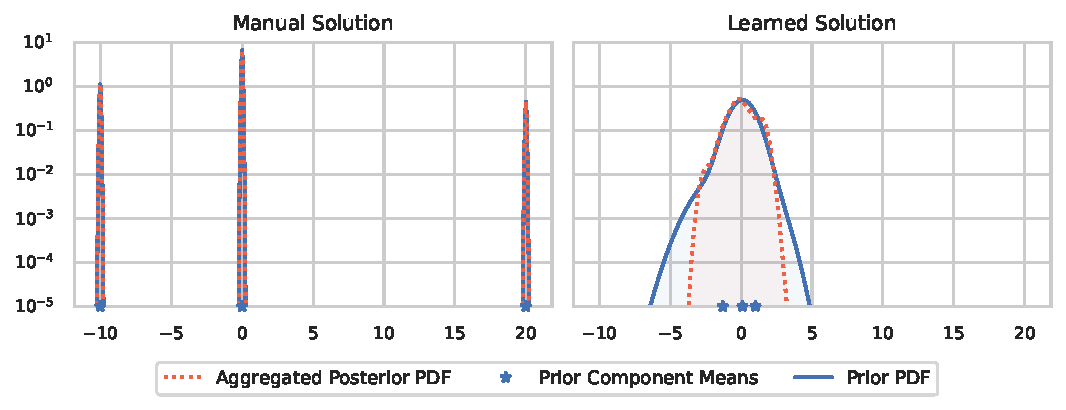
\includegraphics[width=0.85\columnwidth,keepaspectratio]{figures/mlp_plots_appendix.pdf}
    \caption{Manually specified vs. learned distributions for MLP trained with a variational objective on the identity task with an adaptive GMM prior. The aggregated posterior shown in the figure is an equally-weighted mixture of the individual Gaussian posteriors for each MLP weight.} %
    \label{fig:mlp_plots}
\end{figure}



\begin{table}[h!]
\centering
\caption{MLP performance on identity task.}
\vspace{0.15cm}
\scalebox{0.85}{
\label{tab:mlp_results}
\begin{tabular}{
  llccccc
}
\toprule
{\textbf{Objective}} &
{\textbf{Init.}} & {\textbf{KL Coef.}} & {\textbf{KL}} (bits) & {\textbf{Train NLL}} (bits) & {\textbf{Codelength}} (bits) & {\textbf{Accuracy}} \\
\midrule
        MLE Baseline & Random & --- & --- & $8.82$ & --- & $100\%$ \\
        \midrule
        Variational & Random & $1.0$ & $2.87$ & $2.64 \times 10^{3}$ & $2.64 \times 10^{3}$ & $54\%$ \\
                    &        & $10^{-1}$ & $3.19 \times 10^{1}$ & $1.90 \times 10^{3}$ & $1.93 \times 10^{3}$ & $63\%$ \\
                    &        & $10^{-2}$ & $2.24 \times 10^{2}$ & $1.12 \times 10^{2}$ & $3.37 \times 10^{2}$ & $100\%$ \\
                    &        & $10^{-3}$ & $2.88 \times 10^{2}$ & $5.39 \times 10^{1}$ & $3.42 \times 10^{2}$ & $100\%$ \\
                    &        & $10^{-4}$ & $2.98 \times 10^{2}$ & $5.09 \times 10^{1}$ & $3.49 \times 10^{2}$ & $100\%$ \\
        \midrule
        Variational & Manual & $10^{-1}$ & $9.87 \times 10^{1}$ & $ 0.0$ & $9.87 \times 10^{1}$ & $100\%$ \\
        \bottomrule
        
\end{tabular}
}
\end{table}

The results are shown in Table~\ref{tab:mlp_results}, and show similar trends as the Transformer experiments. We see that when starting from a random initialization, the optimization process fails to find a loss comparable to that achieved via manual initialization, indicating poor optimization of the proposed objective. To understand why the randomly initialized models underfit, we can inspect the properties of the learned prior and posterior distributions compared to those from manual initialization. Notably, the prior distribution appears to converge to a unimodal distribution, as visualized in Figure~\ref{fig:mlp_plots}, in contrast to the multimodal prior of the manual solution, with lower-variance components.

\paragraph{Task and network}

Our network is a $2$ layer MLP with $4$ inputs dimensions and $16$ hidden dimensions, that computes the function:
\begin{equation}
    f(x;\theta) = \text{sigmoid}( W^2~\text{ReLU}(W^1(x) + b^1) + b^2)
\end{equation}
with parameters $\theta = (W^1$, $b^1$, $W^2$, $b^2$). 

Our goal is to learn the identity function such that $f(x;\theta) \approx x$ for any binary vector $x \in \{0, 1\}^4$.

\paragraph{Posterior and prior distributions} We parameterize the posterior distribution with an independent Gaussian corresponding to each weight in the MLP. We use a single adaptive GMM prior with 3 components shared across all weights.

\paragraph{Manual solution} A relatively simple ``manual'' solution to the identity task can be constructed by choosing some scalar $\lambda \gg 0$ (we choose $\lambda=20$ in our experiments) and defining the network weights as follows:
\begin{align*}
    W^2 = (W^1)^\top = 
\begin{bmatrix}
\lambda & 0 & 0 & 0 & 0 & \cdots & 0 \\
0 & \lambda & 0 & 0 & 0 & \cdots & 0 \\
0 & 0 & \lambda & 0 & 0 & \cdots & 0 \\
0 & 0 & 0 & \lambda & 0 & \cdots & 0 \\
\end{bmatrix}
&&
    b^1 =
\begin{bmatrix}
-\frac{\lambda}{2} \\
\vdots \\
-\frac{\lambda}{2}
\end{bmatrix}
&&
    b^2 =
\begin{bmatrix}
-\frac{\lambda}{2} \\
\vdots \\
-\frac{\lambda}{2}
\end{bmatrix}
\end{align*}

\paragraph{Training details} The negative log-likelihood of $y$ given $x$ with respect to $\theta$ follows the standard binary cross-entropy loss:
\begin{equation}
    -\log_2 p(y \mid x;\theta) = \sum_{i=1}^4 -y_i \log_2(f(x;\theta)_i) - (1 - y_i) \log_2(1 - f(x;\theta)_i)
\end{equation}
We train the MLP with a variational objective. We specify posterior and prior distributions over $\theta$ as specified above, minimizing the variational objective consisting of the sum of the KL divergence between posterior and prior  distributions, and the expected binary cross entropy loss with respect to sampling weights $\theta$ from the posterior distribution.
We over-sample the space of $2^4$ possible binary vectors of length $4$ to create minibatches for training of $128$ examples.

Sampling, initialization, and training details are similar to the Transformer setting detailed above, except training only required $1,000$ steps. We show a sweep over different KL coefficients in Table~\ref{tab:mlp_results}. 
